\section{Physikalische Grundlagen} % (fold)
\label{sec:grundlagen}

  \subsection{Das $n$-Körper-Problem} % (fold)
  \label{sub:das_n_koerper_problem}

    Das $n$-Körper-Problem betrachtet in seiner allgemeinen Form eine feste Anzahl von Punktmassen, die sich in einem Inertialsystem aufgrund der zwischen ihnen herrschenden Gravitationskraft bewegen.

    \begin{figure}[h]
      \center
      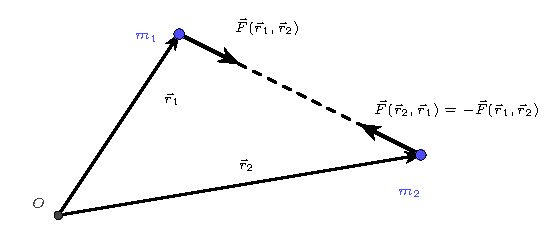
\includegraphics[width=0.95\textwidth]{pictures/gravitational_force.pdf}
      \caption{Die Skizze zeigt die Wirkung der Newtonschen Gravitationskraft anhand zweier Beispielmassen. Die Kraft wirkt entlang der Verbindungslinie der Punktmassen.}
    \end{figure}

    Seien also $n\in\setNatural$ die Anzahl der Punktmassen, $m_i\in\setReal^+$ die Masse und $\function{r_i}{\setReal^+}{\setReal^3}$ die Kurve der $i.$~Punktmasse für alle $i\in\setNatural$ mit $i\leq n$.
    Nach dem zweiten Newtonschen Axiom und dem Newtonschen Gravitationsgesetz mit der Gravitationskonstanten $\gamma$ müssen die Kurven der Punktmassen den folgenden Differentialgleichungen  für alle $i\in\setNatural$ mit $i\leq n$ und alle $t\in\setReal^+$ gehorchen.
    \[
      m_i\ddot{r}_i(t) = \sum_{{j=1,\ j\neq i}}^n \gamma m_im_j \frac{r_j(t)-r_i(t)}{\norm{r_j(t)-r_i(t)}^3}
    \]
    Der Einfachheit halber definieren wir die Beschleunigung $a_i$ einer Punktmasse für alle $i\in\setNatural$ mit $i\leq n$.
    \[
      \function{a_i}{\setReal^{3n}}{\setReal^3}
      \separate
      a_i(r_1,\ldots,r_n)\define \sum_{{j=1,\ j\neq i}}^n \gamma m_j \frac{r_j-r_i}{\norm{r_j-r_i}^3}
    \]
    Für alle $i\in\setNatural$ mit $i\leq n$ vereinfachen sich dann die Differentialgleichungen zu der folgenden Form.
    \[
      \ddot{r}_i(t) = a_i(r_1(t),\ldots,r_n(t))
    \]

    Die Beschleunigung einer jeden Punktmasse hängt damit für jeden gegebenen Zeitpunkt vom gesamten Konfigurationsraum ab.
    Aus diesem Grund erscheint es sinnvoll die gesamte Problemstellung in den Konfigurationsraum zu überführen.
    Hierzu definieren wir als erstes die verallgemeinerte Kurve im Konfigurationsraum.
    \[
      \function{r}{\setReal^+}{\setReal^{3n}}
      \separate
      r(t)\define (r_1(t),\ldots,r_n(t))
    \]
    Der nächste Schritt besteht darin, eine verallgemeinerte Beschleunigung im Konfigurationsraum zu definieren.
    \[
      \function{a}{\setReal^{3n}}{\setReal^{3n}}
      \separate
      a\circ r(t) \define (a_1\circ r(t),\ldots,a_n\circ r(t))
    \]
    Mit diesen Definitionen lässt sich das Problem nun wie folgt für alle $t\in\setReal^+$ formulieren.
    \[
      \ddot{r}(t) = a\circ r(t)
    \]

    Bei dem gegebenen Gleichungssystem handelt es sich um ein gewöhnliches $3n$-dimensionales Differentialgleichungssystem zweiter Ordnung, welches sich, sofern $n\geq 3$, nur für sehr spezielle Fälle analytisch lösen lässt.
    Die später vorgestellten numerischen Integratoren zur Approximation der Lösung eines Anfangswertproblems sind jedoch nur für Differentialgleichungssysteme erster Ordnung anwendbar.
    Deshalb wollen wir zudem eine verallgemeinerte Geschwindigkeit im Konfigurationsraum einführen.
    \[
      \function{v}{\setReal^+}{\setReal^{3n}}
      \separate
      v\define \dot{r}
    \]
    Nach Definition muss damit auch die folgende Gleichung für alle $t\in\setReal^+$ erfüllt sein.
    \[
      \dot{v}(t) = a\circ r(t)
    \]
    Diese Beziehung machen wir uns zu Nutze, um das Problem in den Phasenraum zu überführen.
    Wir definieren eine verallgemeinerte Kurve im Phasenraum, welche zu jedem Zeitpunkt die Orte und Geschwindigkeiten aller Punktmassen beschreibt.
    \[
      \function{p}{\setReal^+}{\setReal^{6n}}
      \separate
      p(t) \define
      \begin{pmatrix}
        r(t) \\ v(t)
      \end{pmatrix}
    \]
    Wie vorher, benötigen wir auch eine verallgemeinerte Beschleunigung im Phasenraum.
    \[
      \function{f}{\setReal^{6n}}{\setReal^{6n}}
      \separate
      f\circ p(t)\define
      \begin{pmatrix}
        v(t) \\ a\circ r(t)
      \end{pmatrix}
    \]
    Aus den Definitionen von $p$ und $f$ folgt dann unmittelbar ein äquivalentes gewöhnliches $6n$-dimensionales Differentialgleichungssystem erster Ordnung in dem für alle $t\in\setReal^+$ das folgende gilt.
    \[
      \dot{p}(t) = f\circ p(t)
    \]

  % subsection das_ (end)

  \subsection{Das Zweikörperproblem} % (fold)
  \label{sub:das_zweikoerperproblem}

    Das Zweikörperproblem ist eine spezielle Form des $n$-Körper-Problems, in welchem $n=2$ gilt und damit nur zwei Punktmassen, die sich gegenseitig beeinflussen, betrachtet werden.
    Das resultierende System von Differentialgleichungen lässt sich analytisch lösen und stellt gerade aus diesem Grund eine Möglichkeit dar numerische Integratoren in Bezug auf ihre Stabilität, Genauigkeit und Geschwindigkeit zu quantifizieren.

    Die Lösung des Zweikörperproblems leitet sich aus dem Einkörperproblem ab, durch die Betrachtung des Schwerpunktsystems und der Einführung der reduzierten Masse.
    Im System selbst gilt die Energie- und Drehimpulserhaltung.
    \[
      E = T + U = \frac{m_1}{2}\norm{v_1}^2 + \frac{m_2}{2}\norm{v_2}^2 - \frac{\gamma m_1m_2}{\norm{r_1-r_2}} = \m{const}
    \]
    \[
      L = L_1 + L_2 = m_1r_1\times v_1 + m_2r_2\times v_2 = \m{const}
    \]
    Hierbei bezeichnet $E$ die Gesamtenergie, $T$ die kinetische Energie, $U$ die potentielle Energie, $L$ den Gesamtdrehimpuls, $L_1$ den Drehimpuls der ersten Punktmasse und $L_2$ den Drehimpuls der zweiten Punktmasse.
    Die Bewegung der Punktmassen findet in einer festen Ebene statt.
    In dieser Ebene kann die Kurve für jede Masse relativ zum Schwerpunkt in Polarkoordinaten unabhängig von der Zeit angegeben werden.
    Jede Bahn stellt einen Kegelschnitt dar.
    \[
      \function{\varrho}{[0,2\pi)}{\setReal^+}
      \separate
      \varrho(\varphi) \define \frac{p}{1+\varepsilon \cos \varphi}
    \]
    Dabei stellt $p$ den Halbparameter (hier ist nicht das Partikelsystem gemeint), $\varepsilon$ die Exzentrizität und $\mu$ die reduzierte Masse dar.
    \[
      p \define \frac{\norm{L}^2}{\gamma \mu^2(m_1+m_2)}
      \separate
      \varepsilon \define \sqrt{1 + \frac{2E\norm{L}^2}{\gamma^2(m_1+m_2)^2\mu^3}}
      \separate
      \mu \define \frac{m_1m_2}{m_1+m_2}
    \]

    Im Schwerpunktsystem beschreiben die Kurven der beiden Massen demanch entweder Ellipsen für $\varepsilon < 1$, Parabeln für $\varepsilon = 1$ oder Hyperbeln für $\varepsilon > 1$.
    Durch Transformation in ein Inertialsystem mit einer vorhandenen Relativgeschwindigkeit im Bezug zum Schwerpunkt, lassen sich bei gebunden Bewegungen auch Zykloiden beobachten.

  % subsection das_zweikörperproblem (end)

  \subsection{Bahnelemente} % (fold)
  \label{sub:bahnelemente}

    Ist die Lösung des Zweikörperproblems beschränkt beziehungsweise gebunden, so bewegen sich wie im vorigen Abschnitt erklärt, die beiden Punktmassen auf Ellipsen im Raum.
    Um die Bewegung einer Punktmasse zu beschreiben, sind, wie aus der theoretischen Mechanik bekannt, sechs Koordinaten notwendig.
    Im kartesischen Inertialsystem, indem auch das Problem formuliert wurde, charakterisieren drei dieser Koordinaten die Position und drei die Geschwindigkeit.
    Dieses System eignet sich für die numerische Simulation.

    In der Astronomie sind diese sechs Koordinaten aber schwer zu messen.
    Aus diesem Grund haben sich die sogenannten Bahnelemente etabliert, die im klassischen Fall ebenfalls durch sechs Parameter $(p,\varepsilon,i,\Omega,\omega,t)$ angegeben werden.
    Hierbei bezeichnet $p$ den Halbparameter, $e$ die Exzentrizität, $i$ die Inklination, $\Omega$ die Winkel des aufsteigenden Knotens, $\omega$ das Argument der Periapsis und $t$ den Zeitbezug.
    Sie beschreiben direkt die Lage und Form der Ellipsen im Raum und eignen sich gerade deshalb zur quantitativen Beschreibungen von Planetenbahnen.
    Zur Beschreibung von Planeten eines Sonnensystems wird statt $p$ auch oft die große Halbachse $a$ verwendet.
    In Abbildung \ref{fig:bahnelemente-scetch} ist noch einmal die Bedeutung einiger Bahnelemente skizziert.

    \urldef{\bahnelementeScetch}\url{https://de.wikipedia.org/wiki/Datei:BahnelementeEllipse.svg}
    \begin{figure}[h]
      \center
      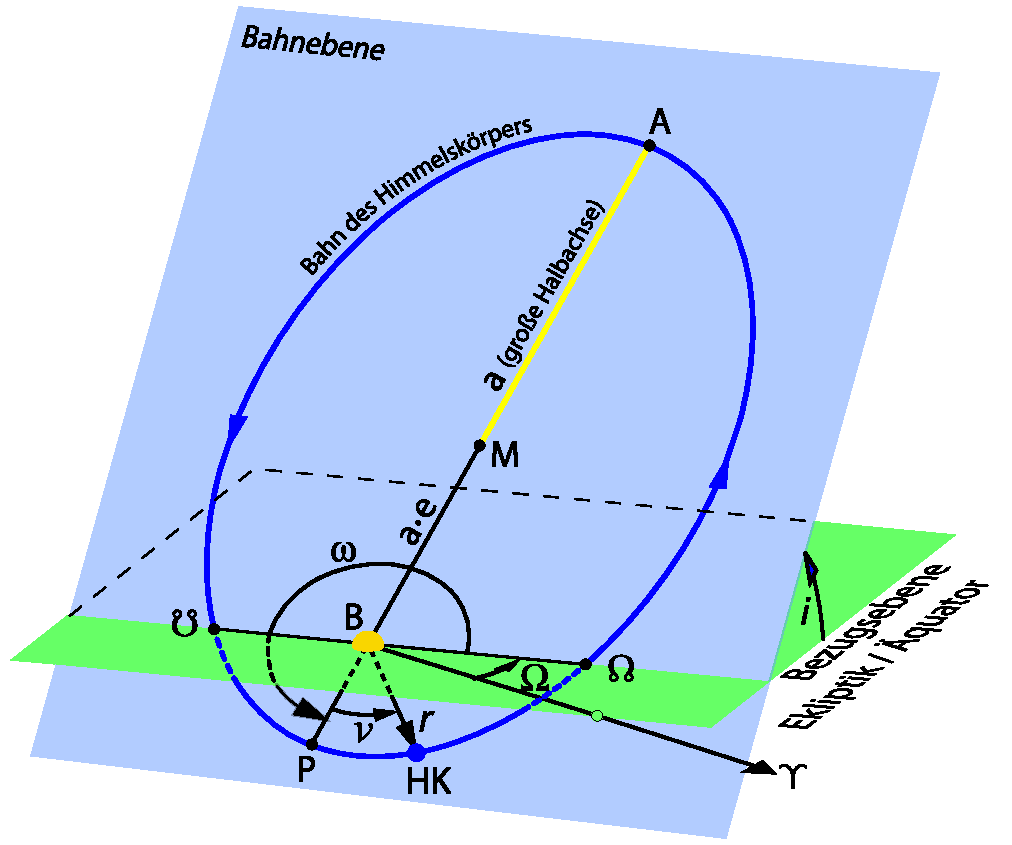
\includegraphics[width=0.95\textwidth]{pictures/BahnelementeEllipse.pdf}
      \caption{Die Skizze zeigt die Bedeutung der klassischen Bahnelemente. \\ Quelle:\\ \bahnelementeScetch}
      \label{fig:bahnelemente-scetch}
    \end{figure}
    Bei der quantitativen Auswertung der Simulation werden wir uns hauptsächlich auf die Parameter $\varepsilon$ und $a$ beziehen.
    Eine Formel zur Berechnung von $\varepsilon$ aus kartesischen Koordinaten wurde bereits in Abschnitt \ref{sub:das_zweikoerperproblem} genannt.
    Aus diesen Koordinaten kann ebenfalls $a$ berechnet werden.
    \[
      a = - \frac{\gamma\mu (m_1+m_2)}{2E}
      \separate
      \varepsilon \define \sqrt{1 + \frac{2E\norm{L}^2}{\gamma^2(m_1+m_2)^2\mu^3}}
    \]
    Die Berechnung der Inklination erfolgt meist über definition einer Bezugsebene, meist die Ekliptik.
    Wenn das Schwerpunktsystem so gewählt wurde, dass sich die Erde ausschließlich in der $xy$-Ebene bewegt, so kann die Inklination $i$ eines beliebigen Himmelskörpers, der den Drehimpuls $L$ besitzt einfach angebeben werden.
    \[
      i = \arcsin \curveBrackets{\frac{L_z}{\norm{L}}}
    \]

  % subsection bahnelemente (end)

  \subsection{Dreikörperproblem} % (fold)
  \label{sub:dreikörperproblem}

    Auch das Dreikörperproblem ist eine spezielle Form des $n$-Körper-Problems, in welchem $n=3$ gilt.
    Es ist im allgemeinen nicht mehr analytisch lösbar.
    Allerdings existieren geschlossene Lösungen für diverse Spezialfälle.
    In Abbildung \ref{fig:dreikoerper} sind beispielhafte Verläufe der Lösungen des Dreikörperproblems dargestellt.

    \urldef{\urldreikoerper}\url{https://tucschneider.files.wordpress.com/2015/03/dreikoerperproblem1.jpg}
    \urldef{\urlmotte}\url{http://scienceblogs.de/astrodicticum-simplex/2015/06/09/unloesbar-und-faszinierend-das-dreikoerperproblem/motte/}
    \begin{figure}[h]
      \center
      \begin{subfigure}{0.49\textwidth}
        \center
        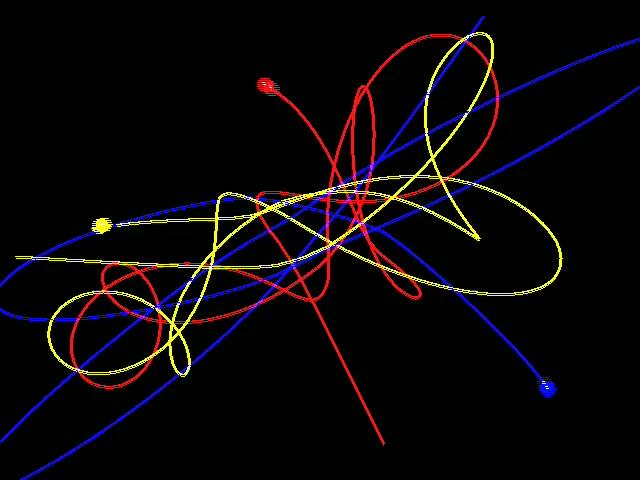
\includegraphics[width=0.8\textwidth]{pictures/dreikoerperproblem1.jpg}
        % \caption{Typische Bahnkurven eines beliebig initialisierten Dreikörperproblems \\ Quelle: \urldreikoerper}
      \end{subfigure}
      \begin{subfigure}{0.49\textwidth}
        \center
        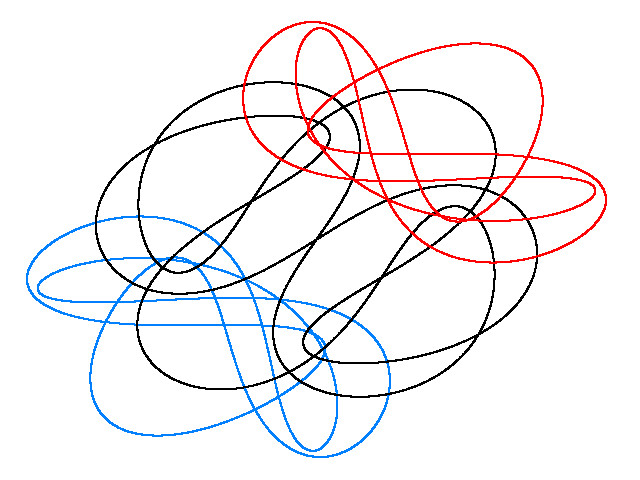
\includegraphics[width=0.8\textwidth]{pictures/motte.jpg}
        % \caption{Typische Bahnkurven eines beliebig initialisierten Dreikörperproblems \\ Quelle: \urldreikoerper}
      \end{subfigure}
      \caption{Die linke Abbildung zeigt die numerische Simulation eines Dreikörperproblems mit zufällig initialisierten Anfangswerten. Die rechte Abbildung zeigt eine spezielle analytische Lösung für die Bahnkurven des Dreikörperproblems. \\ Quellen: \\ \urldreikoerper \\ \urlmotte}
      \label{fig:dreikoerper}
    \end{figure}

  % subsection dreikörperproblem (end)

% section grundlagen (end)